\section{Method} \label{sec:method}

\hline

\note{This was copied from intro. Does it belong here?}

We undertake the task of establishing a consistent regional wave
resource assessment methodology by first pointing out that the wave
resource for a region of water is composed of two parts (Figure
\ref{fig:diagram:west-eez}): 1) the ‘remote resource’, which is the
wave energy created by winds outside the region — e.g., by storms in
the distant open-ocean — that propagates into the region
\citep{gunnQuantifyingGlobalWave2012,
hemerRevisedAssessmentAustralia2017}, and 2) the ‘local resource’,
which is the wave energy created by winds within the region
itself. The majority of existing wave resource assessments have
considered the remote resource only. While neglecting the local
resource may be reasonable for small projects, the fact that it has
been ignored (often implicitly) has raised legitimate questions about the validity of established methodologies, which has led to skepticism and confusion. The primary
objective of this work is to develop a methodology for quantifying
both the remote and local resource explicitly, and thereby bring clarity to the field of regional wave resource assessment.

\begin{figure}[ht]
  \centering
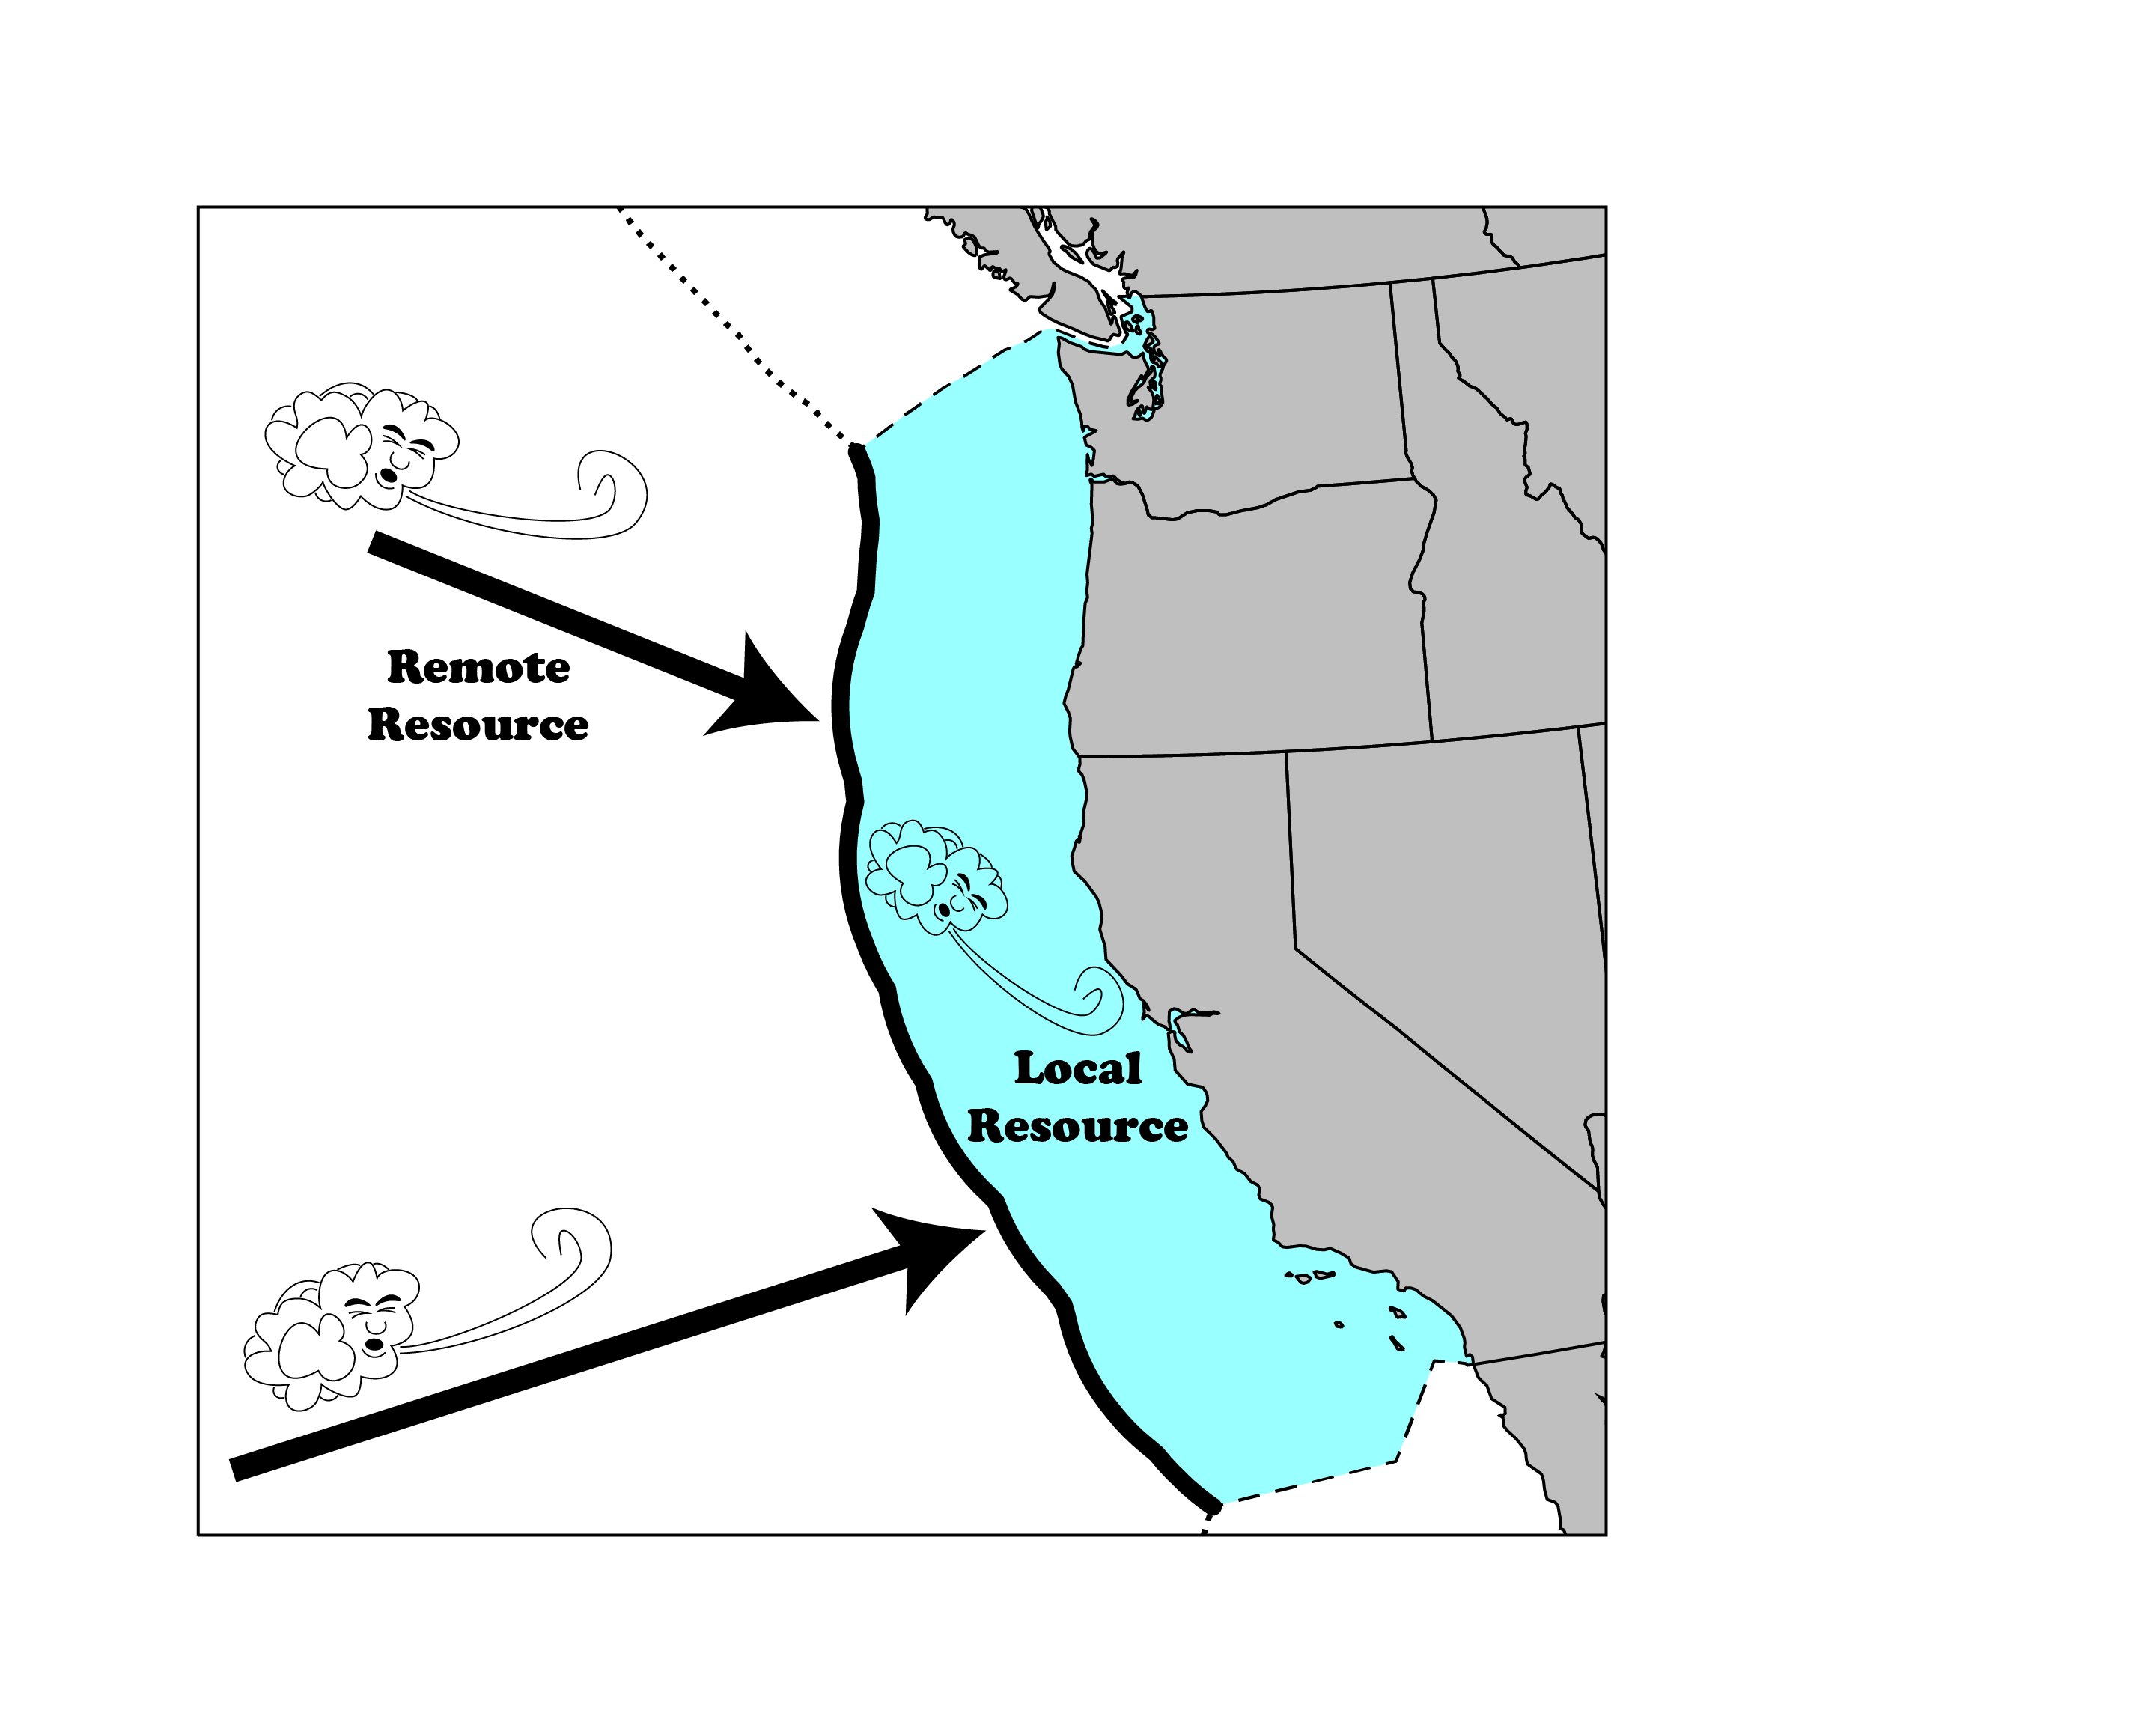
\includegraphics[width=0.9\linewidth]{../diagram/EEZ_contour03_edit01.png}
  \caption{A diagram depicting the U.S. West Coast’s ‘remote’ (arrows) and ‘local’ (cyan region) resource.}
  \label{fig:diagram:west-eez}
\end{figure}

\hline

The overarching goal of this study is to define the wave energy resources and to develop an accurate methodology for estimating the total theoretically available wave resource for a given region. The methodology has been formulated to address the critiques leveled against earlier works, namely: the method should eliminate or at least minimize ``double counting'', and it should also include all sources of wave energy that are legitimately a portion of the region's resource. With these objectives in mind, we propose that regional resource assessment adhere to the following principals:

\begin{itemize}
\item {\bf Follow IEC TS-101 standards for numerical model setup, configuration, and validation.} The IEC standards have done an excellent job of describing detailed guidelines for model setup and procedures for validation. We have followed the ``Class 1, Reconnassance" level here \note{RIGHT?!, or did we follow class 2?, ... or did we not follow IEC?!}, and it is most likely the most relevant class for other regional assessments, but there may be cases where it is desirable to follow class 2 or 3. The one thing that must be added to the IEC guidance is that the model must be configured to output the source terms, so that the `local resource' (below) can be computed.
\item {\bf The total resource is the sum of the remote and local resource.} To our knowledge all prior resource assessments have focused exclusively on the remote resource. The inclusion of the local resource is a means for accounting for the 'recovery' of the wave-field downstream of where energy is extracted.
\begin{itemize}
    \item {\bf Calculate the ``remote resource'' utilizing a one-way dot-product.} this approach has been used in several previous wave resource assessments, but it was not used in the EPRI 2011 assessment \note{Add cites when Zotero integration in overleaf exists.}. This is an fundamental component of wave resource assessment because it avoids the {\em double} counting inherent in the `unit-circle' method used in EPRI 2011, and also avoids {\em under} counting that can occur when using a traditional dot-product. A detailed investigation of the importance of this approach can be found in Appendix \ref{appendix:one-way-method}. \cite{EPRIwaveresource2011}).
    \item {\bf Include the local wave generation:} this consists of quantifying the wave resource generated landward of the boundaries (the EEZ in this study). Considering this part will provide a complete quantification of the resource. Estimates of the resource generated locally has implications to estimating the wave recovery potential, should a significant amount of wave energy is harvested. To the authors' knowledge this has not been considered in previous resource assessments.
\end{itemize}
\item {\bf Extend the assessment to the edge of the region's legal boundaries.} In the case of this analysis, we take this to mean the edge of the U.S. EEZ. This has been done previously by some, but we believe that it should be done consistently for national Resource Assessments. It is important to be consistent with the treatment of the resource across international boundaries. The sum of the resource computed for two regions independently must be the same as if the resource is computed for both regions combined. This sounds rather obvious but should not be overlooked, having a consistent treatment of energy fluxes across borders will result in double counting the total energy.
\end{itemize}


\subsection{Numerical Model} \label{sec:method:model}

Wave resource assessments typically rely on the use of wave model `hindcasts' to estimate the history of the wave field over the region(s) of interest, and then to compute estimates of the theoretical resource from the model output. The reason for this is that in-situ or remote measurements do not cover the oceans with enough resolution, spatially and temporally, to characterize the spatial variations of waves that occur at short scales. 
In this work all wave climate hindcasts are simulated using WAVEWATCH III\textregistered v5.16 \citep{tolmanDistributedmemoryConceptsWave2002,tolmanwavewatch}.

WAVEWATCH III\textregistered (hereafter WW3) is a  well established numerical model that has been implemented successfully in many previous wave resource assessments \citep[e.g.,][]{garcia-medinaWaveResourceAssessment2014,hemerRevisedAssessmentAustralia2017,yangWaveModelTest2017}.
WW3 solves the five-dimensional action balance equation:

\begin{align}
  \frac{DN}{Dt} = \frac{\Src{tot}}{\sigma} = \frac{1}{\sigma}\left ( \Src{in} + \Src{ds} + \Src{brk} + \Src{nl} + \Src{bot} \right )
\end{align}
where $N(t,x,y,\sigma,\theta) \equiv D/\sigma$ is the wave action, $D$ is the variance spectrum, $t$ is time, $x$ and $y$ are the spatial coordinates, $\sigma$ is the radian frequency, and $\theta$ is the direction of wave propagation.
The wave action is conserved in the absence of sinks and sources of energy, their combined effect is represented as $\Src{tot}$.
The models do not include ocean currents so that $\sigma$ (intrinstic frequency) is spatially constant, and therefore wave energy (i.e., variance, $D$) is a conserved quantity (i.e., energy is only gained or lost by the source terms above).

In this study we implement the ``ST4'' physics package option in WW3 to simulate wind energy input ($\Src{in}$) and dissipation due to whitecapping ($\Src{ds}$) \citep{ardhuinObservationSwellDissipation2009}.
The wind forcing (for both the global and regional domains) is taken from NOAA's Climate Forecast System Reanalysis (CFSR) \citep{sahaNCEPClimateForecast2010}. The non-linear quadruplet interactions ($\Src{nl}$) are modeled with the Hasselmann and Hasselmann (\citeyear{hasselmannComputationsParameterizationsNonlinear1985}) formulation. Bottom friction ($\Src{bot}$) and depth induced wave breaking ($\Src{brk}$) are modeled with the JONSWAP Hasselmann etal. \citeyear{hasselmannMeasurementsWindwaveGrowth1973} and Battjes and Janssen \citeyear{battjesEnergyLossSetup1978} models, respectively. Finally, the effect of sea ice is considered by using a time varying mask based on the ice coverage fields from CFSR. Default parameters are used for all formulations.

The WW3 simulations span a 32-year period from January 1, 1979 to December 31, 2010. The first year (1979) is treated as a 'spin-up' year, and is not included in any calculations of resource totals. Variability in the wave climate on timescales longer than the 31-year period included in the average are not considered (i.e., changes in the wave resource due to climate change are not included). The wave spectrum is discretized with 24 equally spaced bins in $\theta$ space and 29 logarithmically spaced frequency bins from 0.035Hz to 0.5Hz with an increment factor of 1.1. 

Model grids and bathymetry come from the NOAA NCEP hindcast Phase 1 mosaic-model \citep{chawla2011wavewatch,chawla201230}. In this system a global model (0.5$^{\circ}$ resolution) drives regional models (10" - 4" resolution) providing complete coverage over the U.S. EEZ with higher resolution focused on shallower waters. This model was reimplemented to store wave spectra and source terms at a high resolution.

Model output is collected at the U.S. EEZ around Alaska (excluding the Arctic Coast), Atlantic Coast, Caribbean Coast (Puerto Rico and U.S. Virgin Islands), Gulf Coast, Hawaii (excluding the Papah$\bar{\text{a}}$naumoku$\bar{\text{a}}$kea Marine National Monument), and the West Coast. Full variance spectra are stored at the U.S. EEZ boundary (at 200 nmi from shore, and along EEZ `borders' with other nation's). Inside the EEZ, directionally integrated source term output is collected at lines of equal distance from shore from 18.5 km (10 nmi) to 351.9 km (190 nmi) every 18.5 kms. Both output types are collected at hourly intervals every 1/6$^{\circ}$ along the defined lines.

This model configuration is mostly aligned with the IEC TS 62600-101 requirements for a reconnaissance class resource assessment. The requirements for physical processes are met with the exception of the inclusion of wave-current interactions and the effect of tides. It is not expected that the tides will influence waves significantly at 18.5 km from shore. Wave-current interactions can be important particularly around the Gulf Stream, thus the exclusion of this must be revisited in future studies. The numerical requirements from IEC TS 62600-101 indicate that spherical coordinates must be used with a minimum temporal resolution of 3h, 25 wave frequency components, 24 azimuthal directions, and a minimum spatial resolution of 5 km. All but the latter are met in this study, the regional models at 4" have a meridional resolution of 7.4 km.


\subsection{Calculate Resource Totals} \label{sec:method:calc}

In this work we propose that the total theoretical wave resource, $R_T$, be defined as a sum of `remote' and `local' components:
\begin{align}
  R_T = R_R + R_L
\end{align}
The remote resource, $R_R$, is the piece of the wave energy resource that has previously been defined as the total wave resource \citep{gunnQuantifyingGlobalWave2012,EPRIwaveresource2011}, while the local resource, $R_L$, has not previously been included in wave resource assessments.

\subsubsection{Remote Resource} \label{sec:method:calc:remote}

The remote resource is computed as a line-integral of the wave energy that fluxes toward the coastline across the EEZ boundary when it is bordered by international waters. 

\begin{align}
  R_R = \rho g \int_{\leez}\iint \delta \, c_g(f) \, \bar{D}(f,\theta) \d f \d \theta \d l
\label{eqn:RR}
\end{align}
Where $c_g(f)$ is the wave group velocity, $\leez$ is the EEZ boundary (integration contour), and $\delta$ is the directionality coefficient which we take to be $\delta = \cos(\theta_n - \theta)$ for waves propagating toward the coastline, and $\delta_1 = 0$ otherwise. $\theta_n$ is the direction of the normal to the integration contour pointing toward the coastline. The `one-way' condition ensures that waves propagating offshore are not {\em subtracted} from the total \citep[]{gunnQuantifyingGlobalWave2012}. A detailed rationalle for the one-way approach to estimating $R_R$ is included in appendix \ref{appendix:one-way-method}. The over-bar denotes a time-average of the wave-variance spectrum over the 31-year period from Jan. 1 1980, through Dec 31, 2010.

The integration contour $\leez$ only includes the segments of the U.S. EEZ that separate U.S. EEZ waters from the open-ocean (hereafter the `EEZ boundary'; thick black line in Figure \ref{fig:diagram:west-eez}), and does not include the EEZ segments that separate one nation's EEZ from that of a neighbor (hereafter the `EEZ borders'; thin dashed lines) \citep[]{flandersmarineinstituteMaritimeBoundariesGeodatabase2018}. This is because wave-energy that fluxes across EEZ borders will be counted -- using the methodology described here -- by the nation from which that resource originated. For example, waves that propagate southward across the Canada-U.S. EEZ border are counted as Canada's resource, and waves that propagate northward across this border are counted as U.S. resource. Either way, these waves will already have been counted in the originating nation's resource, and so including wave fluxes across these borders would only lead to `double counting'.


\subsubsection{Local Resource} \label{sec:method:calc:local}

The local resource is computed as an area-integral of all wave source- and sink-terms, except for bottom friction:

\begin{align}
  R_L &= \rho g \int_{EEZ}\iint \left ( \bar{S}_{in} + \bar{S}_{ds} + \bar{S}_{brk} + \bar{S}_{nl} \right ) \d f \d \theta \d A
\label{eqn:RL}
\end{align}
where $dA$ is differential-area integral of the source terms. Since the model results are output in spherical coordinate system, the coordinates were transformed using an Albers equal area projection before performing the area integral. By performing these projections on a region-by-region basis with carefully chosen projection parameters, this approach introduces $<1\% $ local distortion at the edges of the largest regions (Alaska), and therefore introduces a $\ll 1\%$ error in the total estimate of $R_L$.

This piece has not previously been considered in wave resource assessments, which has led to some criticism in the form of questions like, ``how quickly will the wave-field re-energize down-wave from a wave farm?''  And, ``which contour is the {\em right} contour along-which to compute $R_T = R_R$ (i.e., when $R_L$ is not included in $R_T$)?'' Including $R_L$ in $R_T$ explicitly adds the locally generated wave energy to the total, and therefore addresses these critiques. 

However, because the source terms in \eqref{eqn:RL} depend on the sea-state and the sea-state depends on energy extracted ``up-wave'', there is ambiguity in estimating $R_L$ related to where and when wave energy is extracted by WECs. To address this, we calculate two estimates of $R_L$. The first, `natural local resource' ($R_{L_\circ}$) is calculated from the source-terms where waves from the global domain propagate freely throughout the model domain (i.e., the U.S. EEZ). The second, `potential local resource' ($R_{L_*}$) is calculated from the source-terms when no wave energy propagates across the EEZ boundary. In other words, this latter case can be thought of as a `lake case' that only contains waves generated by winds within the EEZ. 

In all cases we examined, $R_{L_*}$ was found to be greater than $R_{L_\circ}$, which suggests that $R_L$ should be defined as being equal to $R_{L_*}$. However, the scenario of extracting all wave energy at the edge of the EEZ is so hypothetical that it seems unrealistic to use this value to define $R_L$. Therefore, we treat these two estimates of $R_L$ as an uncertainty range for it.

\begin{itemize}
\item source terms are larger when starting with no-waves \note{Is this always true?} \textcolor{green}{I found that sometimes the source terms are larger when extracting 90\% but not by much.}
\item Or is it because sometimes the winds blow {\em against} the waves?
\item Is there an argument here relating to uncertainty in source terms, or is that a {\em different} source of uncertainty?
\item Also, $R_{L_*}$ is {\em so hypothetical} that it is rather unrealistic, so it serves as an upper-bound.
\item There is also some discussion here somewhere about the use of all source-terms, not just $S_{in}$. I think this also relates to the discussion above about whether $R_L = R_{L_*}$ or $R_{L_\circ} < R_L < R_{L_*}$ in the sense that we are making {\em some} assumptions/decisions about what does/does-not count in the `theoretical resource'. \note{Does a discussion of these assumptions/decisions belong here, or in the {\em methods} section?} \textcolor{green}{Yes, stating why bottom friction is not being considered is important. Back at OSU I tested the effect of bottom friction in the model results and were negligible at similar scales to this one. \citep{garcia2013inner}}
\end{itemize}

It is worth noting that -- though directionality is critically important to estimating $R_R$ correctly in \eqref{eqn:RR} -- directionality is not important to estimating $R_L$ correctly (in \eqref{eqn:RL} all directions are weighted equally), only the total energy is. This is because this energy is being added to the wave-field per unit-area (it is not a wave-energy flux), and could theoretically be absorbed by a WEC or array of WECs within the domain before it ever reached a boundary where a line-integral would be appropriate (i.e., when directionality is important).

In WW3, as it is customary in third-generation spectral wave models, the waves are computed over a specified spectral width after which a spectral tail is appended to represent the energy in the high frequencies \citep[e.g.][]{ardhuinObservationSwellDissipation2009}. This frequency cutoff is generally the minimum of the highest described frequency and the cutoff supported by the source term formulations. The simulations in this study are performed with the default high frequency cutoff:

\begin{align}
  f_{c} = \frac{2.5}{T_{m01}}
\end{align}
where $T_{m01}$ is the mean spectral period. The source term integrals are performed for the range where the wave spectrum is actively simulated.

\begin{enumerate}
\item ST4 package (improvement in power density and Hs, but overpredicts energy-period<-- is there a citation for this)\textcolor{green}{I did some searching and didnt find a good discussion about this.}
\item We add all source terms together (except bottom friction), because:
  \begin{itemize}
  \item Questions about accuracy of individual terms \citep{garcia-medinaWaveResourceAssessment2014}
  \item The length-scale over which the input-term acts is similar to that of the dissipation terms.
  \item The non-linear terms transfer energy to lower frequencies (with some losses), and in general the input-term adds energy at frequencies that is above the frequency that most WECs are expected to operate. \note{Is this true? What about small devices/PBE?} \textcolor{green}{The upper limit is 0.5Hz in our study so this is ok}
  \end{itemize}
\item ‘Control volume’ is EEZ surrounding a continent/island. We break this into pieces for each country. I.e.: we don’t include line-integral at boundary between countries.
\end{enumerate}

\subsection{Methodological differences with key previous works}
\label{sec:method:changes}

\note{Also include here some discussion of other RA's? In particular, \citep{gunnQuantifyingGlobalWave2012}, others? Or does this discussion belong in the intro?!}

There are three important pieces of the EPRI 2011 methodology that are different from what is used here:
\begin{enumerate}
\item It includes only the remote resource, because the local resource was not typically considered in wave energy resource assessment at that time
\item It used an integration contour that was much closer to shore (i.e., the 200-m water-depth contour, or 50 nautical-miles from shore, whichever is closer to shore)
\item It did not account for wave directionality, which led to some ``double-counting'' \cite{nationalresearchcouncilEvaluationDepartmentEnergy2013}
\item EPRI 2011 used 52-months, we use 31-years. This is important as pointed out by \cite{yangCharacteristicsVariabilityNearshore2020}.
\end{enumerate}
\note{Do we also need to mention minor differences in method: different model/physics packages? Other?} \textcolor{green}{I do not think so. Source terms will keep changing in the future but this method will still be valid.}


%%% Local Variables:
%%% TeX-master: "wave_res"
%%% End:
